\label{sec:intro}

In recent years, with the development of hardware and algorithm, the intelligence of a single agent has been greatly improved.
The cooperation of agents can expand the capability of a unmanned system [??], and the multi-agent intelligent system is a promising research field.

Multi-robot exploration (MR-Explore) provides location and map for each robot. It is the basic task for many multi-robot applications, such as multi-robot navigation [??] and multi-robot rescue[??].

For the keyword \textit{"robot"}, the feature-point extraction (FE) is a basic component for the visual odometry to estimate the 6 degree of freedom (6-DoF) pose [??].
For the keyword \textit{"multi"}, place recognition (PR) converts the input image into a short representation code, which is a fundamental element to produce candidate place matches between different robots [??].
Recent works use CNN to extract feature-points \cite{detone2018superpoint, simo2015discriminative, yi2016lift} and generate the representation code \cite{arandjelovic2016netvlad, radenovic2018fine}. 
The CNN-based feature-points from \cite{detone2018superpoint} reaches 10\%-30\% higher matching accuracy compared with the popular hand-crafted extraction method, ORB \cite{Mur-Artal:2017281}.
The accuracy of the representation code from CNN-based method \cite{radenovic2018fine} is also ??\% better than the hand-crafted method [??].

\begin{figure}[t]
	\centering
	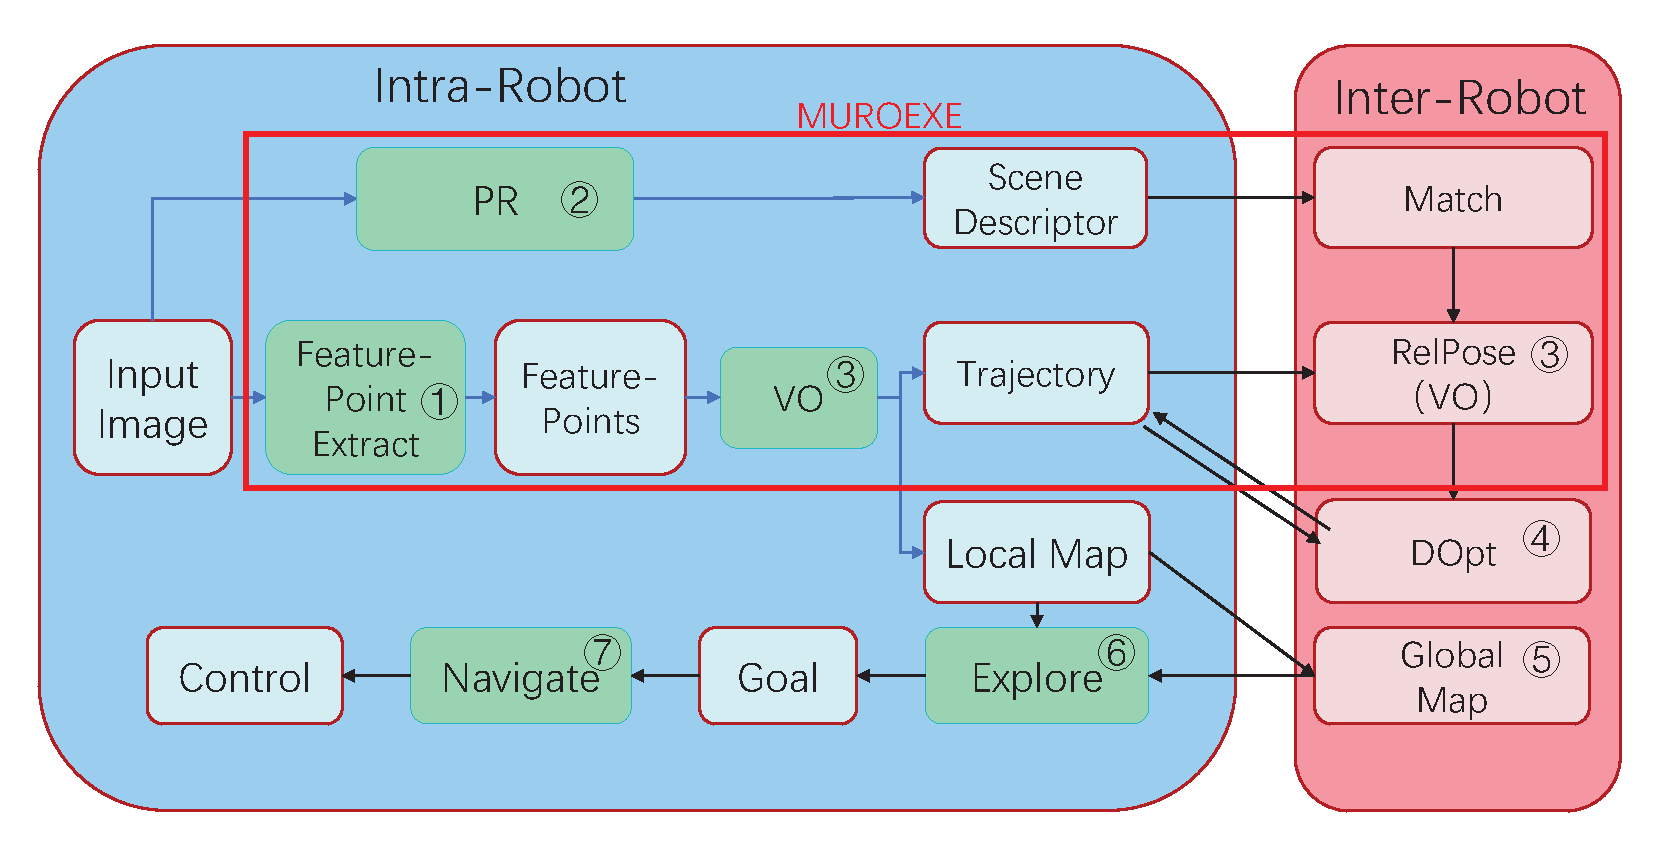
\includegraphics[width=0.99\linewidth]{fig/maexp.eps}
    \caption{
        The modules in MR-Explore. \textcircled{1}\textcircled{3} are basic for a single robot, should be execute every frame. \textcircled{2} generates representation code for some key frames. \textcircled{7}\textcircled{8} are only executed when representation codes are matched across robots and they are latency tolerant.  \textcircled{4}\textcircled{5}\textcircled{6} are for decision and navigation, also latency tolerant.
    }
	\label{fig:maexp}
\end{figure}


\Cref{fig:maexp} illustrates the computation modules in MR-Explore.
Feature-point extraction (\textcircled{1}) and visual odometry (VO, \textcircled{3}) should be performed for each input frame, and should be completed before the next frame. 
Place Recognition (PR, \textcircled{2}) generates the representation code for some key frames, and sends them to other robots. 
When the  representation codes from different robots are matched, optimizaion (\textcircled{7}) and map merging ((\textcircled{8})) are performed to merge the trajectories and maps. \textcircled{4}\textcircled{5}\textcircled{6} are for decision-making and navigation based on the merged maps. 
In this paper, CNN methods are used to realize the Feature-point Extraction (\textcircled{1}) and  Place Recognition (\textcircled{2}).
Besides these two modules, more CNN-based methods, such as semantic segmentation \cite{long2015fully} and object detection \cite{ren2015faster}, can be introduced into embedded moving robots to achieve better accuracy.
Even if only FE and PR are implemented in CNN, the computational complexity reaches 1 TOP/s , which poses a challenge for embedded systems.


\begin{figure*}[t]
    % \flushleft
    \centering
	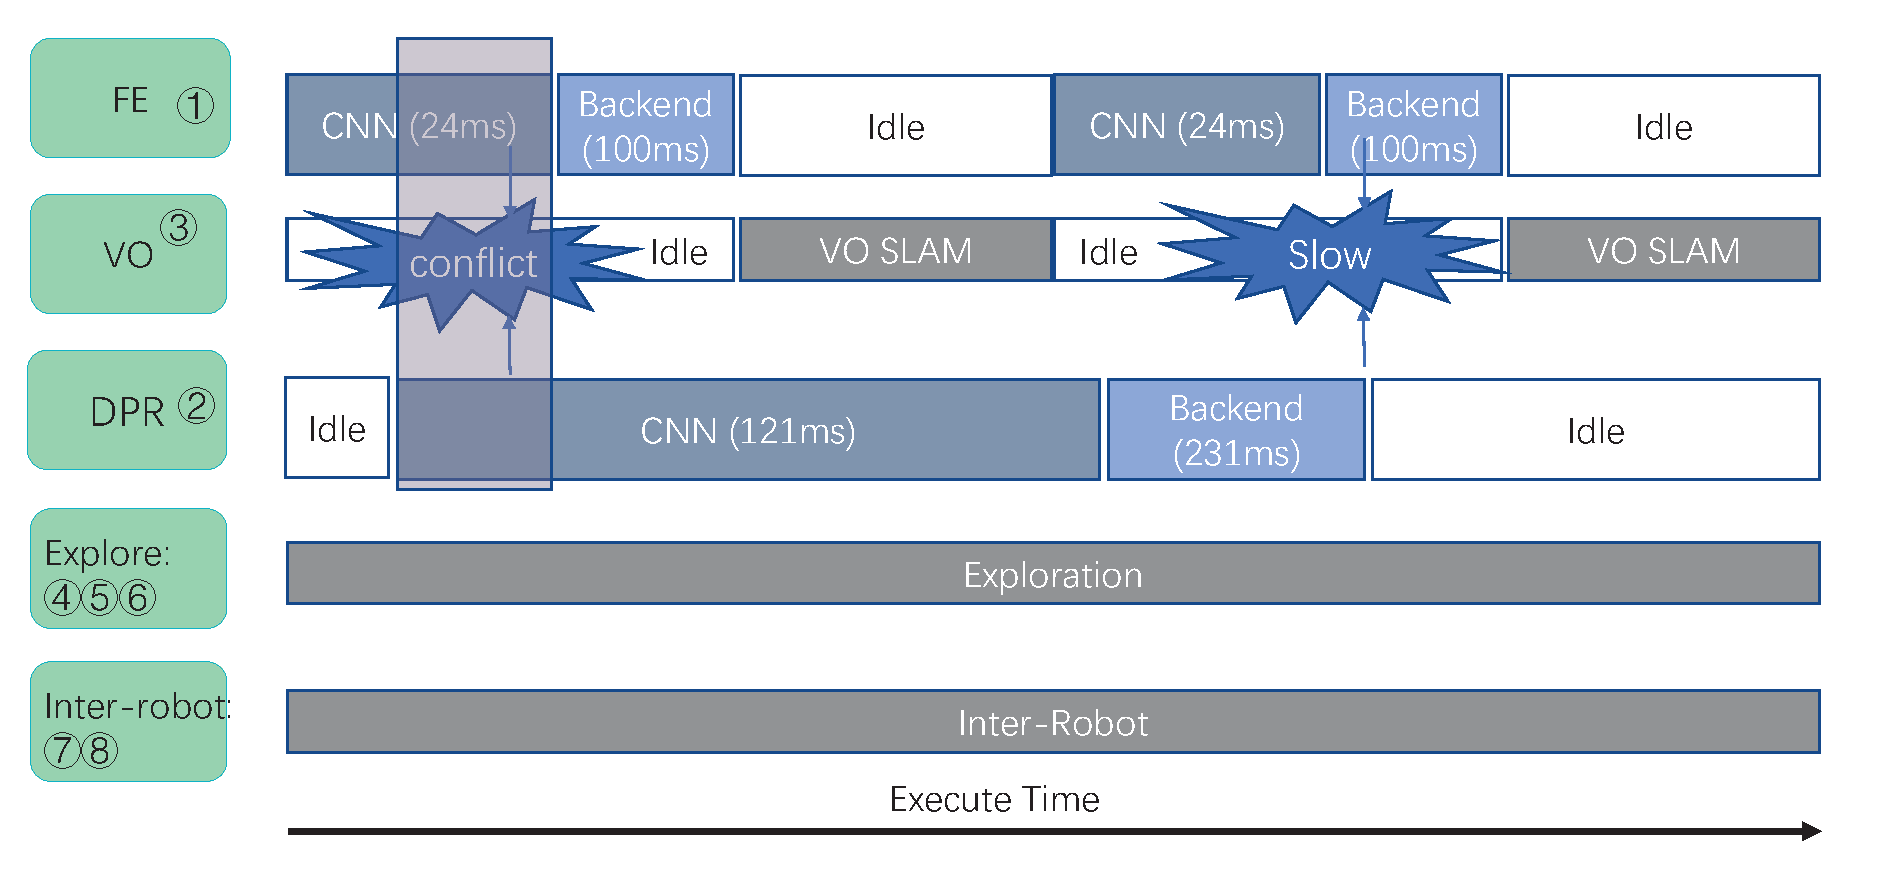
\includegraphics[width=0.7\textwidth]{fig/overalltime.eps} 	
    \caption{
    The overall timeline of MA-Explore.
    }
	\label{fig:overalltime}
\end{figure*}


In recent years, FPGA is becoming a promising platform for algorithm acceleration. Previous works design CNN accelerators on FPGA \cite{yu2018instruction,li_high_2016,qiu2016going,lu_evaluating_2017}. With the help of network quantization and data reuse, the speed of CNN accelerators on embedded FPGA reaches 3TOP/s \cite{lu_evaluating_2017}.
However, previous CNN accelerators are designed and optimized to accelerate a specific CNN. They can not automatically schedule two or more tasks simultaneously. 
The inability of CNN accelerators to support multi-task makes it difficult for researchers in robotics to use embedded FPGA.



The overall timeline of MA-Explore is illustrated in \Cref{fig:overalltime}. 
The threads of FE and PR may need to process CNN at the same time, resulting in hardware resource conflicts. 
In order to facilitate robotic researchers to run several CNN tasks simultaneously on the FPGA accelerators, the accelerator should support the following functions:

\textbf{Multi-thread:} A robot contains many modules including perception, decision-making and control. 
The Robot Operating System (ROS) \cite{quigley2009ros} is a popular middleware fusing different modules from different developers. 
In ROS, each module is considered as an indepentant thread on CPU. 
Different threads should have easy access to the FPGA accelerator.

\textbf{Dynamic Scheduling:} The execution of CNN is depend on other operations, like VO module in \Cref{fig:overalltime}. 
These operations are running at CPU, and the execution time varies with the input data [??] (10ms - 50ms for VO). 
The accelerators cannot predict when to start a task. 
Therefore, the FPGA accelerator should be scheduled dynamically to support irregular task requests from software.

\textbf{Scheduling by priority:} Each module has different priority. The control and perception tasks usually have higher priorities, while the priorities of long-term decision and optimization is lower \cite{RamsauerKLM17}. The critical tasks need to be arranged first on FPGA accelerators.

Besides the CNN backbone, the post-processing of the CNN-based methods are also computation consuming. As illustrated in \Cref{fig:overalltime}, the execution time of post-processing on embedded CPU (~100ms) exceeds that of CNN backbone on the accelerator (30ms), which becomes the bottleneck of the system.


In order to make the CNN accelerator flexible enough for robotic researchers to use, and speed up the post-processing of CNN-based method, we propose a \textit{MU}lti-\textit{RO}bot \textit{EX}ploration \textit{E}ngine ( MUROEXE ). MUROEXE can automatically deploy the MR-Explore on embeded FPGA, with following contributions:

\begin{itemize}[leftmargin = 10 pt]
\item We propose a CNN-based MA-Explore framework based on FPGA. The modules in MUROEXE is designed for ROS \cite{quigley2009ros}, so that the modules can be easily used in other applications.
\item We propose a \textbf{virtual-instruction-based} interrupt method to make the CNN accelerator support dynamic multi-thead scheduling by priority.
\item We optimize the data flow of the post-processing operations. RTL/HLS modules are designed for the optimized post-processing.
\end{itemize}

The rest of this article is organized as follows: \Cref{sec:relate} will introduce the related work. \Cref{sec:cnninterrupt} details the {virtual-instruction-based} interrupt. \Cref{sec:hardsoftcodesign} optimizes the post-processing. \Cref{sec:muroexe} introduce the MUROEXE framework with ROS. Experimental results and analysis are given in \Cref{sec:experiments}. \Cref{sec:conclusion} concludes this article.